% Gerado por scripts/gerar_tabelas.py --- não editar à mão.
\begin{figure}[htbp]
    \centering
    \caption{Estoque de vínculos formais de TI e remuneração mediana, 2007--2025}
    \label{fig:estoque-serie}
    \begin{minipage}[t]{0.49\textwidth}
    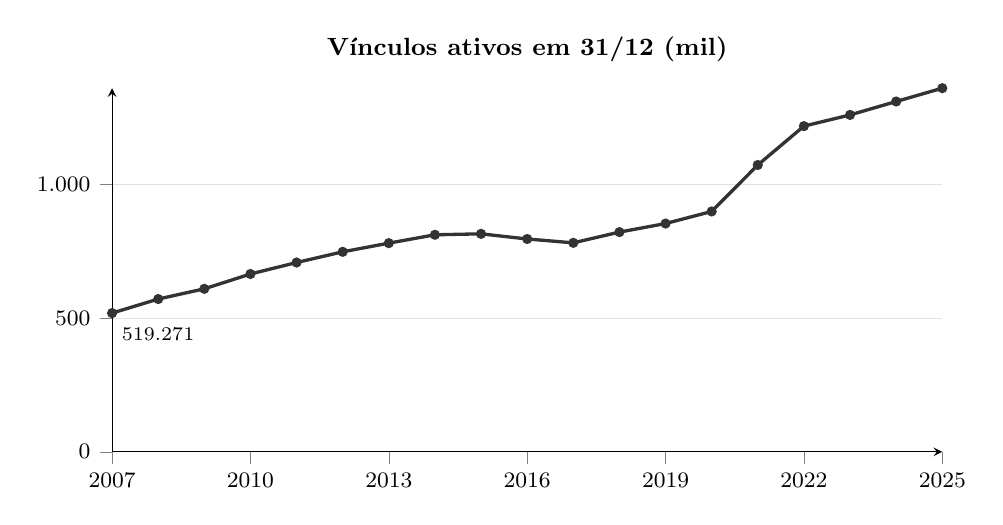
\begin{tikzpicture}
    \begin{axis}[width=\linewidth, height=6.2cm, axis lines=left, tick align=outside,
            ymajorgrids, grid style={black!12}, tick label style={font=\footnotesize},
            label style={font=\footnotesize}, title style={font=\small\bfseries},
            /pgf/number format/use comma, /pgf/number format/1000 sep={.}, title={Vínculos ativos em 31/12 (mil)},
            xmin=2007, xmax=2025, ymin=0, xtick distance=3,
            x tick label style={/pgf/number format/1000 sep={}}]
        \addplot[very thick, black!80, mark=*, mark size=1.2pt] coordinates {(2007,519.3) (2008,571.9) (2009,610.2) (2010,665.6) (2011,708.6) (2012,748.7) (2013,781.2) (2014,812.4) (2015,816.0) (2016,796.7) (2017,782.3) (2018,822.5) (2019,854.5) (2020,899.8) (2021,1073.7) (2022,1219.2) (2023,1261.1) (2024,1311.3) (2025,1361.2)};
        \node[font=\scriptsize, anchor=north west, yshift=-2pt] at (axis cs:2007,519.3) {519.271};
        \node[font=\scriptsize, anchor=south east] at (axis cs:2025,1361.2) {1.361.231};
    \end{axis}
    \end{tikzpicture}
    \end{minipage}\hfill
    \begin{minipage}[t]{0.49\textwidth}
    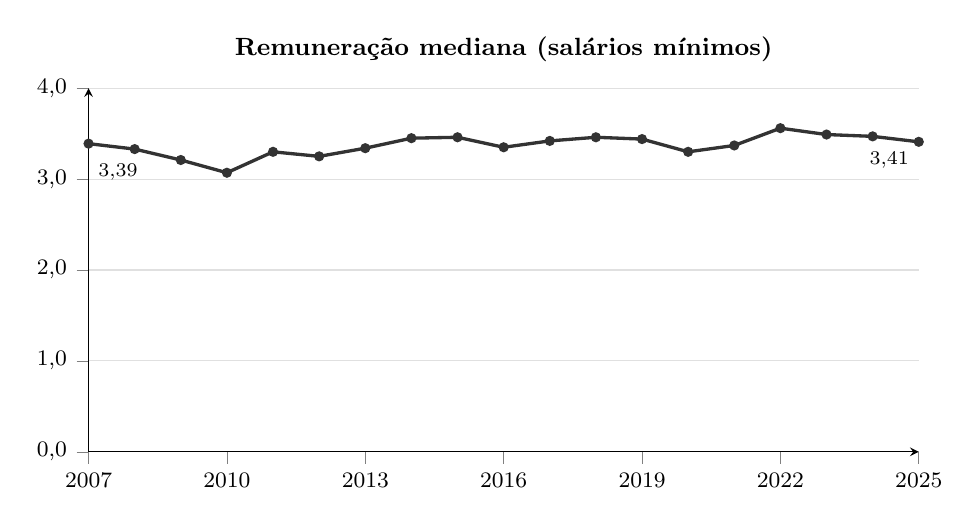
\begin{tikzpicture}
    \begin{axis}[width=\linewidth, height=6.2cm, axis lines=left, tick align=outside,
            ymajorgrids, grid style={black!12}, tick label style={font=\footnotesize},
            label style={font=\footnotesize}, title style={font=\small\bfseries},
            /pgf/number format/use comma, /pgf/number format/1000 sep={.}, title={Remuneração mediana (salários mínimos)},
            xmin=2007, xmax=2025, ymin=0, ymax=4, xtick distance=3,
            x tick label style={/pgf/number format/1000 sep={}},
            y tick label style={/pgf/number format/.cd, use comma, fixed, fixed zerofill, precision=1}]
        \addplot[very thick, black!80, mark=*, mark size=1.2pt] coordinates {(2007,3.39) (2008,3.33) (2009,3.21) (2010,3.07) (2011,3.3) (2012,3.25) (2013,3.34) (2014,3.45) (2015,3.46) (2016,3.35) (2017,3.42) (2018,3.46) (2019,3.44) (2020,3.3) (2021,3.37) (2022,3.56) (2023,3.49) (2024,3.47) (2025,3.41)};
        \node[font=\scriptsize, anchor=north west, yshift=-4pt] at (axis cs:2007,3.39) {3,39};
        \node[font=\scriptsize, anchor=north east] at (axis cs:2025,3.41) {3,41};
    \end{axis}
    \end{tikzpicture}
    \end{minipage}
    \\[4pt]
    {\footnotesize Valores anuais na \autoref{tab:estoque-serie}, no \autoref{apend:series}. }Fonte: Autoria própria, a partir da camada Gold.
\end{figure}
